% Commands
% Document class
\documentclass[a4paper, 11pt]{report}
\usepackage[utf8]{inputenc}

% Table of contents
\usepackage[nottoc,notlof,notlot]{tocbibind} % including references
\setcounter{tocdepth}{2} % depth
\setcounter{secnumdepth}{3} % section numbering depth

% Miscellaneous
\usepackage{fullpage} % different margins
\usepackage{hyperref} % links
\usepackage[binary-units=true]{siunitx} % MB, GB, etc.
\usepackage{pdfpages} % import PDFs
\usepackage{verbatim} % multi-line comments

% Checkmarks and xmarks
\usepackage{amssymb}
\usepackage{pifont}
\definecolor{green}{RGB}{0,176,80}
\newcommand{\cmark}{{\color{green}\textbf{\ding{51}}} }
\definecolor{red}{RGB}{222,0,0}
\newcommand{\xmark}{{\color{red}\textbf{\ding{55}}} }

% Adding a dot at the end of paragraph titles
\let\originalparagraph\paragraph
\renewcommand{\paragraph}[2][.]{\originalparagraph{#2#1}}

% Glossaries and acronyms
% section,numberedsection=autolabel
\usepackage[acronym,toc]{glossaries} % package
% General
\newacronym{rm}{RM}{Resource Manager}
\newacronym{rmf}{RMF}{Resource Management Framework}
\newacronym{vm}{VM}{Virtual Machine}
\newacronym{inp}{INP}{In-Network Processing}
\newacronym{nfv}{NFV}{Network Function Virtualization}
\newacronym{sdn}{SDN}{Software Defined Networking}
\newacronym{tor}{ToR}{Top of Rack}
\newacronym{hpc}{HPC}{High Performance Computing}
\newacronym{dht}{DHT}{Distributed hash table}

% Programming
\newacronym{api}{API}{Application Programming Interface}
\newacronym{mpi}{MPI}{Message Passing Interface}
\newacronym{rpc}{RPC}{Remote Procedure Call}

% Resource models
\newacronym{vc}{VC}{Virtual Cluster}
\newacronym{voc}{VOC}{Virtual Oversubscribed Cluster}
\newacronym{tivc}{TIVC}{Time-Interleaved Virtual Cluster}
\newacronym{tag}{TAG}{Tenant Application Graph}

% SHArP
\newacronym{an}{AN}{Aggregation Node}
\newacronym{am}{AM}{Aggregation Manager}
\newacronym{tca}{TCA}{Target Channel Adapter}
\newacronym{qp}{QP}{Queue Pair}
\newglossaryentry{ibm}{
    name=IBM,
    description=IBM\textsuperscript{\textregistered}
}
\newglossaryentry{switchib2}{
    name=Mellanox's SwitchIB-2,
    description=Mellanox's SwitchIB-2\textsuperscript{TM}
}

% Apache Hadoop YARN
\newglossaryentry{apache}{
    name=Apache,
    description=Apache\textsuperscript{TM}
}
\newglossaryentry{hadoop}{
    name=Apache Hadoop,
    description=\glsdesc{apache} Hadoop\textsuperscript{\textcopyright}
}
\newglossaryentry{yarn_full}{
    name=Apache Hadoop YARN,
    description=\glsdesc{hadoop} YARN \texorpdfstring{\cite{yarn}}{}
}
\newglossaryentry{yarn}{
    name=Apache YARN,
    description=\glsdesc{apache} YARN \texorpdfstring{\cite{yarn}}{}
} % acronyms
% Glossary definition
\newglossary*{resources}{Resources glossary}

\newglossaryentry{resource:physical}{
    type=resources,
    name=Physical resource,
    text=physical resource,
    description={physical hardware component of limited availability within a physical machine}
}

    \newglossaryentry{resource:physical:server}{
        type=resources,
        name=Physical server resource,
        text=physical server resource,
        parent=resource:physical,
        description={resource of a physical server machine}
    }
    
    \newglossaryentry{resource:physical:switch}{
        type=resources,
        name=Physical switch resources,
        text=physical switch resources,
        parent=resource:physical,
        description={resource of a physical switche, network accelerator, middle-box and of every kind of network device originally intended to forward packets}
    }
    
\newglossaryentry{resource:logical}{
    type=resources,
    name=Logical resource,
    text=logical resource,
    description={logical representation of a physical resource}
}

    \newglossaryentry{resource:logical:server}{
        type=resources,
        name=Logical server resource,
        text=logical server resource,
        parent=resource:logical,
        description={virtualized server physical resource, often implemented by means of a \gls{vm}, container or an entire physical server}
    }
    
    \newglossaryentry{resource:logical:switch}{
        type=resources,
        name=Logical switch resource,
        text=logical switch resource,
        parent=resource:logical,
        description={logical representation of a physical switch resource not mapped to any physical switch device}
    }
    
    \newglossaryentry{resource:logical:edge}{
        type=resources,
        name=Logical edge resource,
        text=logical edge resource,
        parent=resource:logical,
        description={properties of virtual connections between two logical resources, e.g., bandwidth, latency, etc}
    }
    
\newglossaryentry{resource:composite}{
    type=resources,
    name=Composite,
    text=composite,
    description={template describing a high-level logical component.
        It can be made out of other composites and/or logical resources.}
}

    \newglossaryentry{resource:composite:server}{
        type=resources,
        name=Server composite,
        text=server composite,
        parent=resource:composite,
        description={composite describing a high-level server component, e.g., \textit{web server}, \textit{databases}, etc}
    }
    
    \newglossaryentry{resource:composite:inp}{
        type=resources,
        name=\gls{inp} composite,
        text=\texorpdfstring{\gls{inp}}{INP} composite,
        parent=resource:composite,
        description={composite describing a high-level \gls{inp} application, e.g., \textit{IncBricks} \cite{incbricks}, \textit{NetChain} \cite{netchain}, etc}
    }
    
\newglossaryentry{model}{
    type=resources,
    name=Resource model,
    text=resource model,
    description={model capable of describing composites and logical resources.
        The model exposed to tenants and the one internally used by the \gls{rm} could be different}
}

    \newglossaryentry{model:tenant}{
        type=resources,
        name=Tenant-side model,
        text=tenant-side model,
        parent=model,
        description={resource model exposed to tenants by the system \gls{api}}
    }
    
    \newglossaryentry{model:rm}{
        type=resources,
        name=\gls{rm}-side model,
        text=\texorpdfstring{\gls{rm}}{RM}-side model,
        parent=model,
        description={resource model internally used by the placement algorithm in order to allocate logical resources}
    } % resources glossary
\makeglossaries % computing the glossary and acronyms list

% In-line lists
\usepackage[inline]{enumitem}
\newlist{mylist}{enumerate*}{1}
\setlist[mylist]{label=(\roman*)}

% References sections
\renewcommand{\sectionautorefname}{\S}
\renewcommand{\subsectionautorefname}{\S}
\renewcommand{\subsubsectionautorefname}{\S}
\renewcommand\bibname{References}

% Capitalized references
\usepackage{cleveref}

% Footnotes with symbols
\usepackage[symbol]{footmisc}
\renewcommand{\thefootnote}{\fnsymbol{footnote}}

% Document start
\begin{document}
\noindent

% This is the thesis summary document
\newcommand*\THESISSUMMARY{}

% Title
% \begin{titlepage}
%     \begin{center}
%         \vspace*{7cm}
 
%         \Huge
%         \textbf{Data center resource management for in-network processing}
 
%         \vspace{1cm}
        
%         \huge
%         Marco Micera
 
%         \vfill
 
%         \LARGE
%         \textit{Politecnico di Torino, TU Darmstadt}
%     \end{center}
% \end{titlepage}

\begin{ThesisTitlePage}
    % Per cambiare la dicitura sopra la lista dei laureandi decommentare
    % la riga seguente, cambiando le 4 parole in modo consistente
    %
    \TitoloListaCandidati{Studente,Studenti,Studentessa,Studentesse}
    %
    \ateneo{Politecnico di Torino, TU Darmstadt}
    %
    % Non tutte le università hanno un nome proprio
    % \nomeateneo{DAUIN - Department of Control and Computer Engineering, DSP - Distributed Systems Programming Group}
    %
    \struttura[III]{Matematica, Fisica e~Scienze Naturali}
    %\Materia{Remote sensing}
    \titolo{Data center resource management for in-network processing}% per la laurea quinquennale e il dottorato
    % \sottotitolo{Metodo dei satelliti medicei}% per la laurea quinquennale e il dottorato
    %
    %%%%%%% Corso degli studi
    \corsodilaurea{Computer Engineering}% per la laurea
    
    %%%%%%% L'eventuale numero di matricola va fra parentesi quadre
    %\show\Candidato
    \def\Candidato{Candidate}
    %\show\Candidato
    \candidato{Marco \textsc{Micera}}[253157] 
    %\secondocandidato{Evangelista \textsc{Torricelli}}[123457]
    
    %%%%%%% Relatori o supervisori
    %
    \def\Relatori{Supervisors}
        \relatore{Prof. Fulvio Risso}
        \secondorelatore{Prof. Patrick Eugster}
        \terzorelatore{M.Sc. Marcel Bl{\"o}cher}
    % 
    %%%%%%% Per mettere altri relatori consultare toptesi-it.pdf
    
    %%%%%%% Tutore
    % \tutoreaziendale{dott.\ ing.\ Giovanni Giacosa}
    % \NomeTutoreAziendale{Supervisore aziendale\\Centro Ricerche FIAT}
    
    %%%%%%% Seduta dell'esame
    %\sedutadilaurea{Agosto 1615}
    %%%%%%%% oppure:
    \sedutadilaurea{\textsc{Anno~accademico} 2019-2020}% 
    
    %%%%%%% Logo della sede
    % \logosede{logodue}% 
    \end{ThesisTitlePage}


%
% Compliant to the thesis summary needed by the ICM/ETF board secretary
%
% 1. title, graduand name, supervisors names
% 2. thesis purpose and brief description of the research area
% 3. personal contribution and results obtained
%
% 3 pages max
%

% Sections
\section{Info}
\textbf{Title}: Data center resource management for in-network processing\\
\textbf{Graduand name}: Marco Micera\\
\textbf{Supervisors}: Prof. Fulvio Risso \footnote[2]{\label{polito} Computer Networks Group, Politecnico di Torino, Italy}, Prof. Patrick Eugster \footnote[3]{\label{tuda} Distributed Systems Programming Group, Technische Universit{\"a}t Darmstadt, Germany}, M.Sc. Marcel Bl{\"o}cher \footref{tuda}\\
\textbf{Research areas}: cloud computing, distributed systems, data centers

\section{Thesis purpose}
Data centers distributed systems can nowadays make use of in-network computation to improve several factors: \textsc{Daiet} \cite{daiet} inventors claim to achieve a 86.9\%-89.3\% traffic reduction by performing data aggregation entirely in the network data plane.
Other solutions like \textsc{NetChain} \cite{netchain} and \textsc{IncBricks} \cite{incbricks} let programmable switches store data and process queries in order to cut end-to-end latency.
It is now even possible to provide guarantees to applications with specific requirements: for instance, \textsc{CloudMirror} \cite{cloudmirror} enables applications to reserve a minimum bandwidth.\par
For the time being, it seems that there is still no valid resource allocation algorithm that takes into account the presence of a network having a data plane that is (in part o completely) capable of basic \gls{inp} operations.
The objective of this thesis is to model and evaluate an \gls{api} through which applications can ask for resources in a data center exploiting \gls{inp} capabilities while providing guarantees (e.g., bandwidth).

% \subsection{Modeling \texorpdfstring{\glsentryshort{inp}}{INP} resources}
% One of the two goals of this Master's thesis consists in investigating how to model \gls{inp} resources and how to integrate them into RMs.
In order to offer \gls{inp} services to a tenant application, the latter should be able to ask for \gls{inp} resources through an \gls{api}.
To do that, \gls{inp} resources must be modeled not only to support currently existing \gls{inp} solutions such as \cite{daiet} \cite{netchain} \cite{incbricks} \cite{sharp}, but also future ones. 
It may also be convenient to derive a single model to describe both server and \gls{inp} resources.

Classic tenant application requests can often be modeled as a key-value data structure.
CloudMirror \cite{cloudmirror} requires a \gls{tag} as an input, which is a directed graph where each vertex represents an application component and links' weights represent the minimum requested bandwidth.
One possible model could be based on a \gls{tag}, describing network resources and \gls{inp} services as vertexes or links.
Tenant applications could either use the same model used within the data center or a simplified one, adding another level of abstraction.


% \subsection{\texorpdfstring{\glsentryshort{inp}}{INP}-aware \texorpdfstring{\glsentrylongpl{rm}}{Resource Managers}} \label{inp_aware_rms}
% \glsreset{rm}
% \glsreset{rm}
In order for everything to work, a network-aware placement algorithm in the \glsentrylong{rm} should be able to consider \gls{inp} and \glslink{resource:logical:server}{server} resources conjunctly: this brings new challenges in the field of resource management as there are currently no \glspl{rm} doing this.
One problem that could arise is due to the fact that \gls{inp} resources are typically very limited in a data center: \autoref{conclusions} will argue the importance of an \gls{rm} which is flexible enough to propose alternatives based on the current utilization of \gls{inp} and \glslink{resource:logical:server}{server} resources, since one kind of \glslink{resource:physical}{physical resource} type can become the bottleneck for the other.


\section{Personal contribution}

\subsection{System design} \label{system_design}
The thesis introduces an overall system design comprising all steps needed to translate \glslink{resource:logical}{resources} expressed using the \gls{model:tenant} to \glslink{resource:physical}{physical ones} so that they could eventually be placed.
The whole system design is depicted in \autoref{compositestophysical}.
The system also introduces the concept of \gls{resource:composite}:
\say{\glsdesc{resource:composite}}
\Glspl{resource:composite} can be translated into \glspl{resource:logical} by means of a \textit{template database}.

\newsavebox\compositestophysical \savebox\compositestophysical{
    % trim = left, bottom, right, top
    \includegraphics[page=6, clip, trim=0.35cm 2.1cm 0.35cm 5cm, width=0.95\textwidth]{design/model/presentation.pdf}
}
\begin{figure}[!htb]
    \centering
    \usebox{\compositestophysical}
    \caption{From the \gls{model:tenant} to \glspl{resource:physical}}
    \label{compositestophysical}
\end{figure}

\subsubsection{\texorpdfstring{\Glsentrytext{resource:composite}}{Composite}s translation methods}
\Glspl{resource:composite} can have multiple properties specifying some application requirements or constraints.
\ifdefined\THESISSUMMARY \else

\fi
A first approach called \textit{passive mapping} would require tenant applications to explicitly express internal \glspl{resource:composite}' properties that \textbf{directly} affect their equivalent expressed in terms of just \glspl{resource:logical}.
\ifdefined\THESISSUMMARY \else
\autoref{passivemapping} shows an example of a tenant application explicitly specifying the chain length of its IncBricks \cite{incbricks} \gls{resource:composite} and the bandwidth demands $B_1$ and $B_2$ towards and outwards it, respectively.
\fi
This, of course, increases the expressiveness of the tenant application with the cost of making the interface more complex to
\ifdefined\THESISSUMMARY
use.
\else
use \xmark \ref{requirements:model:tenant:verbosity}.
\fi
\ifdefined\THESISSUMMARY \else
\begin{figure}[!htb]
    \centering
    \usebox{\passivemapping}
    \caption{Passive template mapping}
    \label{passivemapping}
\end{figure}
\fi
\ifdefined\THESISSUMMARY \else

\fi
With the opposite approach (\textit{active mapping}), tenant applications do not have to specify internal \glspl{resource:composite}' properties, but instead more abstract performance goals.
These high-level \glspl{resource:composite}' goals will be then translated by the \gls{rm}.
\ifdefined\THESISSUMMARY \else
An example of this translation is showed in \autoref{passivemapping}, where the requested tuple rate is transformed accordingly into topology and bandwidth constraints.
\fi
This approach simplifies the interface exposed to tenant applications by not letting them taking care of internal \glspl{resource:composite}' properties that might be unknown to
\ifdefined\THESISSUMMARY
developers.
\else
developers \cmark \ref{requirements:model:tenant:verbosity}.
\fi

\ifdefined\THESISSUMMARY \else
\begin{figure}[!htb]
    \centering
    \usebox{\activemapping}
    \caption{Active template mapping}
    \label{activemapping}
\end{figure}
\fi


\subsection{Resource model}
Alongside the system previously described (\autoref{system_design}), the design chapter of this thesis introduces a resource model proposal that is capable of describing existing \gls{inp} solutions as well as future ones: the \gls{etag}.
\newsavebox\tagmodfigure \savebox\tagmodfigure{
    % trim = left, bottom, right, top
    \includegraphics[page=3, clip, trim=0.6cm 0.6cm 0.6cm 0.6cm, width=0.95\textwidth]{design/model/variants.pdf}
}
% Commands
% Document class
\documentclass[a4paper, 11pt]{report}
\usepackage[utf8]{inputenc}

% Table of contents
\usepackage[nottoc,notlof,notlot]{tocbibind} % including references
\setcounter{tocdepth}{2} % depth
\setcounter{secnumdepth}{3} % section numbering depth

% Miscellaneous
\usepackage{fullpage} % different margins
\usepackage{hyperref} % links
\usepackage[binary-units=true]{siunitx} % MB, GB, etc.
\usepackage{pdfpages} % import PDFs
\usepackage{verbatim} % multi-line comments

% Checkmarks and xmarks
\usepackage{amssymb}
\usepackage{pifont}
\definecolor{green}{RGB}{0,176,80}
\newcommand{\cmark}{{\color{green}\textbf{\ding{51}}} }
\definecolor{red}{RGB}{222,0,0}
\newcommand{\xmark}{{\color{red}\textbf{\ding{55}}} }

% Adding a dot at the end of paragraph titles
\let\originalparagraph\paragraph
\renewcommand{\paragraph}[2][.]{\originalparagraph{#2#1}}

% Glossaries and acronyms
% section,numberedsection=autolabel
\usepackage[acronym,toc]{glossaries} % package
% General
\newacronym{rm}{RM}{Resource Manager}
\newacronym{rmf}{RMF}{Resource Management Framework}
\newacronym{vm}{VM}{Virtual Machine}
\newacronym{inp}{INP}{In-Network Processing}
\newacronym{nfv}{NFV}{Network Function Virtualization}
\newacronym{sdn}{SDN}{Software Defined Networking}
\newacronym{tor}{ToR}{Top of Rack}
\newacronym{hpc}{HPC}{High Performance Computing}
\newacronym{dht}{DHT}{Distributed hash table}

% Programming
\newacronym{api}{API}{Application Programming Interface}
\newacronym{mpi}{MPI}{Message Passing Interface}
\newacronym{rpc}{RPC}{Remote Procedure Call}

% Resource models
\newacronym{vc}{VC}{Virtual Cluster}
\newacronym{voc}{VOC}{Virtual Oversubscribed Cluster}
\newacronym{tivc}{TIVC}{Time-Interleaved Virtual Cluster}
\newacronym{tag}{TAG}{Tenant Application Graph}

% SHArP
\newacronym{an}{AN}{Aggregation Node}
\newacronym{am}{AM}{Aggregation Manager}
\newacronym{tca}{TCA}{Target Channel Adapter}
\newacronym{qp}{QP}{Queue Pair}
\newglossaryentry{ibm}{
    name=IBM,
    description=IBM\textsuperscript{\textregistered}
}
\newglossaryentry{switchib2}{
    name=Mellanox's SwitchIB-2,
    description=Mellanox's SwitchIB-2\textsuperscript{TM}
}

% Apache Hadoop YARN
\newglossaryentry{apache}{
    name=Apache,
    description=Apache\textsuperscript{TM}
}
\newglossaryentry{hadoop}{
    name=Apache Hadoop,
    description=\glsdesc{apache} Hadoop\textsuperscript{\textcopyright}
}
\newglossaryentry{yarn_full}{
    name=Apache Hadoop YARN,
    description=\glsdesc{hadoop} YARN \texorpdfstring{\cite{yarn}}{}
}
\newglossaryentry{yarn}{
    name=Apache YARN,
    description=\glsdesc{apache} YARN \texorpdfstring{\cite{yarn}}{}
} % acronyms
% Glossary definition
\newglossary*{resources}{Resources glossary}

\newglossaryentry{resource:physical}{
    type=resources,
    name=Physical resource,
    text=physical resource,
    description={physical hardware component of limited availability within a physical machine}
}

    \newglossaryentry{resource:physical:server}{
        type=resources,
        name=Physical server resource,
        text=physical server resource,
        parent=resource:physical,
        description={resource of a physical server machine}
    }
    
    \newglossaryentry{resource:physical:switch}{
        type=resources,
        name=Physical switch resources,
        text=physical switch resources,
        parent=resource:physical,
        description={resource of a physical switche, network accelerator, middle-box and of every kind of network device originally intended to forward packets}
    }
    
\newglossaryentry{resource:logical}{
    type=resources,
    name=Logical resource,
    text=logical resource,
    description={logical representation of a physical resource}
}

    \newglossaryentry{resource:logical:server}{
        type=resources,
        name=Logical server resource,
        text=logical server resource,
        parent=resource:logical,
        description={virtualized server physical resource, often implemented by means of a \gls{vm}, container or an entire physical server}
    }
    
    \newglossaryentry{resource:logical:switch}{
        type=resources,
        name=Logical switch resource,
        text=logical switch resource,
        parent=resource:logical,
        description={logical representation of a physical switch resource not mapped to any physical switch device}
    }
    
    \newglossaryentry{resource:logical:edge}{
        type=resources,
        name=Logical edge resource,
        text=logical edge resource,
        parent=resource:logical,
        description={properties of virtual connections between two logical resources, e.g., bandwidth, latency, etc}
    }
    
\newglossaryentry{resource:composite}{
    type=resources,
    name=Composite,
    text=composite,
    description={template describing a high-level logical component.
        It can be made out of other composites and/or logical resources.}
}

    \newglossaryentry{resource:composite:server}{
        type=resources,
        name=Server composite,
        text=server composite,
        parent=resource:composite,
        description={composite describing a high-level server component, e.g., \textit{web server}, \textit{databases}, etc}
    }
    
    \newglossaryentry{resource:composite:inp}{
        type=resources,
        name=\gls{inp} composite,
        text=\texorpdfstring{\gls{inp}}{INP} composite,
        parent=resource:composite,
        description={composite describing a high-level \gls{inp} application, e.g., \textit{IncBricks} \cite{incbricks}, \textit{NetChain} \cite{netchain}, etc}
    }
    
\newglossaryentry{model}{
    type=resources,
    name=Resource model,
    text=resource model,
    description={model capable of describing composites and logical resources.
        The model exposed to tenants and the one internally used by the \gls{rm} could be different}
}

    \newglossaryentry{model:tenant}{
        type=resources,
        name=Tenant-side model,
        text=tenant-side model,
        parent=model,
        description={resource model exposed to tenants by the system \gls{api}}
    }
    
    \newglossaryentry{model:rm}{
        type=resources,
        name=\gls{rm}-side model,
        text=\texorpdfstring{\gls{rm}}{RM}-side model,
        parent=model,
        description={resource model internally used by the placement algorithm in order to allocate logical resources}
    } % resources glossary
\makeglossaries % computing the glossary and acronyms list

% In-line lists
\usepackage[inline]{enumitem}
\newlist{mylist}{enumerate*}{1}
\setlist[mylist]{label=(\roman*)}

% References sections
\renewcommand{\sectionautorefname}{\S}
\renewcommand{\subsectionautorefname}{\S}
\renewcommand{\subsubsectionautorefname}{\S}
\renewcommand\bibname{References}

% Capitalized references
\usepackage{cleveref}

% Footnotes with symbols
\usepackage[symbol]{footmisc}
\renewcommand{\thefootnote}{\fnsymbol{footnote}}

% Document start
\begin{document}
\noindent

% Title
% \begin{titlepage}
%     \begin{center}
%         \vspace*{7cm}
 
%         \Huge
%         \textbf{Data center resource management for in-network processing}
 
%         \vspace{1cm}
        
%         \huge
%         Marco Micera
 
%         \vfill
 
%         \LARGE
%         \textit{Politecnico di Torino, TU Darmstadt}
%     \end{center}
% \end{titlepage}

\begin{ThesisTitlePage}
    % Per cambiare la dicitura sopra la lista dei laureandi decommentare
    % la riga seguente, cambiando le 4 parole in modo consistente
    %
    \TitoloListaCandidati{Studente,Studenti,Studentessa,Studentesse}
    %
    \ateneo{Politecnico di Torino, TU Darmstadt}
    %
    % Non tutte le università hanno un nome proprio
    % \nomeateneo{DAUIN - Department of Control and Computer Engineering, DSP - Distributed Systems Programming Group}
    %
    \struttura[III]{Matematica, Fisica e~Scienze Naturali}
    %\Materia{Remote sensing}
    \titolo{Data center resource management for in-network processing}% per la laurea quinquennale e il dottorato
    % \sottotitolo{Metodo dei satelliti medicei}% per la laurea quinquennale e il dottorato
    %
    %%%%%%% Corso degli studi
    \corsodilaurea{Computer Engineering}% per la laurea
    
    %%%%%%% L'eventuale numero di matricola va fra parentesi quadre
    %\show\Candidato
    \def\Candidato{Candidate}
    %\show\Candidato
    \candidato{Marco \textsc{Micera}}[253157] 
    %\secondocandidato{Evangelista \textsc{Torricelli}}[123457]
    
    %%%%%%% Relatori o supervisori
    %
    \def\Relatori{Supervisors}
        \relatore{Prof. Fulvio Risso}
        \secondorelatore{Prof. Patrick Eugster}
        \terzorelatore{M.Sc. Marcel Bl{\"o}cher}
    % 
    %%%%%%% Per mettere altri relatori consultare toptesi-it.pdf
    
    %%%%%%% Tutore
    % \tutoreaziendale{dott.\ ing.\ Giovanni Giacosa}
    % \NomeTutoreAziendale{Supervisore aziendale\\Centro Ricerche FIAT}
    
    %%%%%%% Seduta dell'esame
    %\sedutadilaurea{Agosto 1615}
    %%%%%%%% oppure:
    \sedutadilaurea{\textsc{Anno~accademico} 2019-2020}% 
    
    %%%%%%% Logo della sede
    % \logosede{logodue}% 
    \end{ThesisTitlePage}


%
% Compliant to the summary needed by the ICM/ETF board secretary
%
% 1. title, graduand name, supervisors names
% 2. thesis purpose and brief description of the research area
% 3. personal contribution and results obtained
%

% Sections
\section{Info}
\textbf{Title}: Data center resource management for in-network processing\\
\textbf{Graduand}: Marco Micera\\
\textbf{Supervisors}: Prof. Fulvio Risso  \footnote[2]{\label{polito} Computer Networks Group, Politecnico di Torino, Italy}, Prof. Patrick Eugster \footnote[3]{\label{tuda} Distributed Systems Programming Group, Technische Universit{\"a}t Darmstadt, Germany}, M.Sc. Marcel Bl{\"o}cher \footref{tuda}\\
\textbf{Research areas}: cloud computing, distributed systems, in-network processing

\section{Thesis purpose}
Data centers distributed systems can nowadays make use of in-network computation to improve several factors: \textsc{Daiet} \cite{daiet} inventors claim to achieve a 86.9\%-89.3\% traffic reduction by performing data aggregation entirely in the network data plane.
Other solutions like \textsc{NetChain} \cite{netchain} and \textsc{IncBricks} \cite{incbricks} let programmable switches store data and process queries in order to cut end-to-end latency.
It is now even possible to provide guarantees to applications with specific requirements: for instance, \textsc{CloudMirror} \cite{cloudmirror} enables applications to reserve a minimum bandwidth.\par
For the time being, it seems that there is still no valid resource allocation algorithm that takes into account the presence of a network having a data plane that is (in part o completely) capable of basic \gls{inp} operations.
The objective of this thesis is to model and evaluate an \gls{api} through which applications can ask for resources in a data center exploiting \gls{inp} capabilities while providing guarantees (e.g., bandwidth).

\subsection{Modeling \texorpdfstring{\glsentryshort{inp}}{INP} resources}
One of the two goals of this Master's thesis consists in investigating how to model \gls{inp} resources and how to integrate them into RMs.
In order to offer \gls{inp} services to a tenant application, the latter should be able to ask for \gls{inp} resources through an \gls{api}.
To do that, \gls{inp} resources must be modeled not only to support currently existing \gls{inp} solutions such as \cite{daiet} \cite{netchain} \cite{incbricks} \cite{sharp}, but also future ones. 
It may also be convenient to derive a single model to describe both server and \gls{inp} resources.

Classic tenant application requests can often be modeled as a key-value data structure.
CloudMirror \cite{cloudmirror} requires a \gls{tag} as an input, which is a directed graph where each vertex represents an application component and links' weights represent the minimum requested bandwidth.
One possible model could be based on a \gls{tag}, describing network resources and \gls{inp} services as vertexes or links.
Tenant applications could either use the same model used within the data center or a simplified one, adding another level of abstraction.


\subsection{\texorpdfstring{\glsentryshort{inp}}{INP}-aware \texorpdfstring{\glsentrylongpl{rm}}{Resource Managers}} \label{inp_aware_rms}
\glsreset{rm}
In order for everything to work, a network-aware placement algorithm in the \glsentrylong{rm} should be able to consider \gls{inp} and \glslink{resource:logical:server}{server} resources conjunctly: this brings new challenges in the field of resource management as there are currently no \glspl{rm} doing this.
One problem that could arise is due to the fact that \gls{inp} resources are typically very limited in a data center: this thesis argues the importance of an \gls{rm} which is flexible enough to propose alternatives based on the current utilization of \gls{inp} and \glslink{resource:logical:server}{server} resources, since one kind of \glslink{resource:physical}{physical resource} type can become the bottleneck for the other.

\section{Personal contribution and obtained results}

\subsection{System design}

\subsubsection{\texorpdfstring{\Glsentrytext{resource:composite}}{Composite}s translation methods}

\subsection{Resource model}

\subsection{Generic groups}

\subsection{Simulation}

\subsubsection{Results}

\subsection{Conclusions}

% References
\bibliographystyle{abbrv}
\bibliography{../thesis/utility/references}

% Document end
\end{document}

\subsection{Generic groups}
\glsreset{sdn}
\glsreset{nfv}
\glsreset{inp}
\Cref{background} introduced how resources can be managed in a data center (\autoref{rm_background}) and different network techniques such as \gls{sdn} (\autoref{sdn_background}), \gls{nfv} (\autoref{nfv_background}) and \gls{inp} (\autoref{inp_background}).
This chapter aims to dig into the details of these systems and to extract common patterns between similar \gls{inp} solutions to then derive a model capable of fully describing \gls{inp} resources.

\section{Obtained results}

\subsection{Simulation}
\glsreset{sdn}
\glsreset{nfv}
\glsreset{inp}
\Cref{background} introduced how resources can be managed in a data center (\autoref{rm_background}) and different network techniques such as \gls{sdn} (\autoref{sdn_background}), \gls{nfv} (\autoref{nfv_background}) and \gls{inp} (\autoref{inp_background}).
This chapter aims to dig into the details of these systems and to extract common patterns between similar \gls{inp} solutions to then derive a model capable of fully describing \gls{inp} resources.
The scheduler used for this evaluation uses a simple greedy placement algorithm that cycles through all \glspl{resource:physical} every time a job needs to be scheduled.
It tries to allocate as many tasks as possible on the same \glslink{resource:physical}{physical machine} simply by
\begin{mylist}
    \item checking the amount of available numerical resources and
    \item performing the \textit{properties} check for switch tasks
    \ifdefined\THESISSUMMARY
    (i.e., whether a \glslink{resource:physical:switch}{physical switch} supports a specific \gls{resource:composite:inp})
    \else
    as described in \autoref{simulator_switch_resources}
    \fi
\end{mylist}.
Experiments ran on Dell C6420 servers on CloudLab \cite{cloudlab}, simulating a 3-days long workload. % FIXME sim time
The simulated data center architecture is a fat-tree with
\ifdefined\THESISSUMMARY
4 pods.
\else
$k=4$ (\autoref{dc_architecture}).
\fi

\ifdefined\THESISSUMMARY \else
\subsection{Metrics}
\fi
These simulations focus on the average \glslink{resource:physical}{resource} utilization in the data center for all dimensions.
Different simulations vary in the ratio between the number of tenant requests including \gls{inp} composites over the overall amount of requests.

\subsection{Results}
Results show how easily one kind of \glslink{resource:physical}{physical resource} can become the bottleneck for the other, and that the ratio of incoming \gls{inp} requests is a key factor for the overall data center utilization.
Ideally, all types of \glspl{resource:physical} in data center should be fully utilized.
When plotting the less relatively-used \glslink{resource:physical}{resource} dimension as a function of the percentage on \gls{inp} requests, a peak around a certain percentage of \gls{inp} requests appears.
This remarks the importance of a scheduler which can reject \gls{inp} requests and propose their server-only equivalent when needed (e.g., high switch utilization).

\subsection{Conclusions}
\glsreset{sdn}
\glsreset{nfv}
\glsreset{inp}
\Cref{background} introduced how resources can be managed in a data center (\autoref{rm_background}) and different network techniques such as \gls{sdn} (\autoref{sdn_background}), \gls{nfv} (\autoref{nfv_background}) and \gls{inp} (\autoref{inp_background}).
This chapter aims to dig into the details of these systems and to extract common patterns between similar \gls{inp} solutions to then derive a model capable of fully describing \gls{inp} resources.

\subsubsection{Fully \texorpdfstring{\glsentryshort{inp}}{INP}-aware \texorpdfstring{\glsentryshort{rm}}{RM} features}
% "On Tackling" has the con of not placing server and switches conjunctly, during the same round
\paragraph{Conjunct placement}
\ifdefined\THESISSUMMARY \else
As mentioned in \autoref{network_resources-aware_rms},
\fi
\cite{ontackling} considers both \glslink{resource:logical:switch}{server} and \glspl{resource:logical:switch} during allocation, but it does not place them during the same scheduling round.
The drawback of not scheduling these two kinds of \glslink{resource:logical}{resources} conjunctly causes the placement algorithm to derive a sub-optimal
\ifdefined\THESISSUMMARY
placement.
\else
placement, as explained in \autoref{network_resources-aware_rms}.

\fi
Ideally, an \gls{rm} should allocate a job considering its \glslink{resource:logical:switch}{server} and \glspl{resource:logical:switch} at the same time, i.e., during the same placement round.

% RMs should propose server-only alternatives
\paragraph{\gls{inp} alternatives}
\ifdefined\THESISSUMMARY
Results showed
\else
The results reported in \autoref{results} show
\fi
an underutilization of \glspl{resource:physical} depending on the number of tenant requests containing \glspl{resource:composite:inp}.
\ifdefined\THESISSUMMARY \else

\fi
To maximize the (relative) minimum \gls{resource:physical} utilization, the \gls{rm} would need to adjust the ratio of \gls{inp} requests over \glslink{resource:logical:server}{servers}-only ones.
With the assumption that \glspl{resource:physical:switch} can become the bottleneck of whole the system more rapidly (e.g., less \glslink{resource:physical:switch}{switches} than \glslink{resource:physical:server}{servers} in a fat-tree with $k>5$ or for the scarceness of
\ifdefined\THESISSUMMARY
\glslink{resource:logical:switch}{switch resources}
\else
\glspl{cu}
\fi
in general),
\glspl{rm} should be able to propose alternatives to \glspl{resource:composite:inp} made out of \glspl{resource:logical:server} or \glspl{resource:composite:server} only, as soon as \glspl{resource:physical:switch} become heavily utilized.
Those alternatives could be stored, for instance, in the same \textit{template database}
\ifdefined\THESISSUMMARY \else
(\autoref{system_design_overview})
\fi
used to translate \glspl{resource:composite:inp} into a set of \glspl{resource:logical:switch}.


% \subsubsection{Open problems}
% Some of the important metrics used in \autoref{evaluation} are still unknown due to the lack of operational \glspl{rm} that handle \gls{inp} requests.

% STC
\glsreset{stc}
In order for \glspl{rm} to be able to propose alternatives, the performance improvement of all \gls{inp} solutions in the \textit{template database} must be reduced to a single number that represents the reduction of \glslink{resource:logical:server}{server} tasks after the introduction of an \gls{resource:composite:inp}: the \gls{stc}.

% Number of needed switch tasks
Moreover, there should be a precise way of determining the number of \glslink{resource:logical:switch}{switch} tasks needed to implement an \gls{resource:composite:inp}, and this could depend on a lot of factors like the set nodes to which the \gls{resource:composite:inp} is connected to in the \gls{etag}, its high-level properties, etc.

% INP service and batch composites
Another key aspect to consider is the type of life cycle that different \gls{inp} solutions might have.
Similarly to \glslink{resource:logical:server}{server} requests, batch (short-term) and service (long-term) jobs may need different scheduling policies.
\gls{inp} solutions should also be categorized on the same basis, e.g., NetChain \cite{netchain} as a service \gls{resource:composite:inp} (since most likely it will be running for a long time, serving multiple \glslink{resource:logical:server}{server} tasks) and Daiet \cite{daiet} or SHArP \cite{sharp} as a batch one.


% References
\bibliographystyle{abbrv}
{\footnotesize\bibliography{../thesis/utility/references}}

% Document end
\end{document}